\documentclass[11pt,a4paper]{article}

% ---------- Packages ----------
\usepackage[utf8]{inputenc}
\usepackage[T1]{fontenc}
\usepackage{lmodern}
\usepackage[french]{babel}
\usepackage[margin=2.5cm]{geometry}
\usepackage{amsmath, amssymb}
\usepackage{graphicx}
\usepackage{booktabs}      % requis par les tableaux exportés par pandas
\usepackage{caption}
\usepackage{float}
\usepackage{microtype}
\usepackage[hidelinks]{hyperref}

\graphicspath{{resultats/}}
\captionsetup{font=small, labelfont=bf}
\setlength{\parindent}{0pt}
\setlength{\parskip}{0.6em}

% Raccourcis
\newcommand{\mux}{\mu_x}
\newcommand{\muhat}{\hat{\mu}_x}

\title{LACTU2030 -- Assurance vie\\ Projet de groupe 2026-2027}
\author{% À COMPLÉTER : noms des membres du groupe
Julien Delmotte \and Binôme}
\date{30 novembre 2026}

\begin{document}
\maketitle
\tableofcontents
\newpage

% =====================================================================
\section{Modélisation statique de la mortalité}
% =====================================================================

\subsection{Données et modèle}

Nous utilisons les données belges de la \emph{Human Mortality Database} (nombres de décès $D_x$ et expositions $E_x$, par âge, année et sexe), pour les années 2020 et 2023 et les âges de 30 à 105 ans, soit 76 âges par jeu de données. Le taux brut est
\[
\muhat = \frac{D_x}{E_x}.
\]
Les quatre jeux d'analyse sont notés F2020, F2023 (femmes) et H2020, H2023 (hommes). Le modèle paramétrique ajusté est
\[
\mux = \exp\!\Big( a + b\,x + c\,(x-70)\,\mathbf 1_{\{x\ge 70\}} \Big),
\]
où $a$ est un niveau de base, $b$ la pente de $\log \mux$ avant 70 ans, et $c$ la modification de cette pente après 70 ans (la pente vaut $b+c$ au-delà de 70 ans). Deux jeux de paramètres $(a,b,c)$ sont estimés pour chaque sexe, l'un pour 2020 et l'autre pour 2023.

\textbf{Hypothèse de travail.} Nous supposons $\mux$ constant sur chaque intervalle $[x,x+1[$. La probabilité de survie sur une année vaut alors $p_x = e^{-\mux}$ et la survie sur $k$ années vaut
\[
{}_kp_x = \exp\!\Big(-\sum_{j=0}^{k-1}\mu_{x+j}\Big).
\]
% À COMPLÉTER si besoin : justifier ce choix (la consigne parle de ``mortality probabilities'').

\subsection{Ajustement par minimisation de l'erreur quadratique moyenne}

\subsubsection{Méthode}

Les paramètres sont estimés en minimisant l'erreur quadratique moyenne entre les taux \emph{bruts} et les taux du modèle (et non entre leurs logarithmes) :
\[
\mathrm{MSE}(a,b,c)=\frac{1}{76}\sum_{x=30}^{105}\Big(\muhat-\mux(a,b,c)\Big)^2 .
\]
La minimisation est numérique (algorithme de Nelder-Mead, avec des tolérances très serrées). Le point de départ est obtenu par une régression linéaire de $\log\muhat$ sur $(1,\ x,\ \max(x-70,0))$, qui a la même structure que le modèle. Nous avons vérifié que les minima obtenus sont les mêmes avec d'autres algorithmes et d'autres points de départ, ainsi qu'avec une implémentation indépendante en R.

\subsubsection{Résultats}

Les paramètres estimés sont donnés dans le tableau~\ref{tab:param_mse}.

\begin{tabular}{lrrr}
\toprule
 & a & b & c \\
\midrule
F2020 & -26.7794 & 0.3333 & -0.2466 \\
F2023 & -14.9629 & 0.1569 & -0.0601 \\
H2020 & -16.9266 & 0.1963 & -0.1120 \\
H2023 & -18.4355 & 0.2170 & -0.1431 \\
\bottomrule
\end{tabular}


\textbf{Remarque importante.} Les paramètres obtenus pour F2020 ($a\approx-26{,}8$, $b\approx0{,}333$, $c\approx-0{,}247$) peuvent sembler surprenants. Ils correspondent pourtant bien au minimum de la MSE. En effet, les erreurs sont mesurées en valeur absolue : aux grands âges $\muhat$ est de l'ordre de $0{,}1$ à $0{,}5$ et les carrés des écarts valent $10^{-3}$ à $10^{-2}$, tandis qu'à 30 ans $\muhat\approx 2\cdot10^{-4}$ et l'écart au carré est de l'ordre de $10^{-8}$. Les grands âges pèsent donc environ $10^{5}$ fois plus dans le critère que les âges jeunes, et le minimum sacrifie l'ajustement des âges jeunes (voir la figure~\ref{fig:log}).

\begin{figure}[htbp]
  \centering
  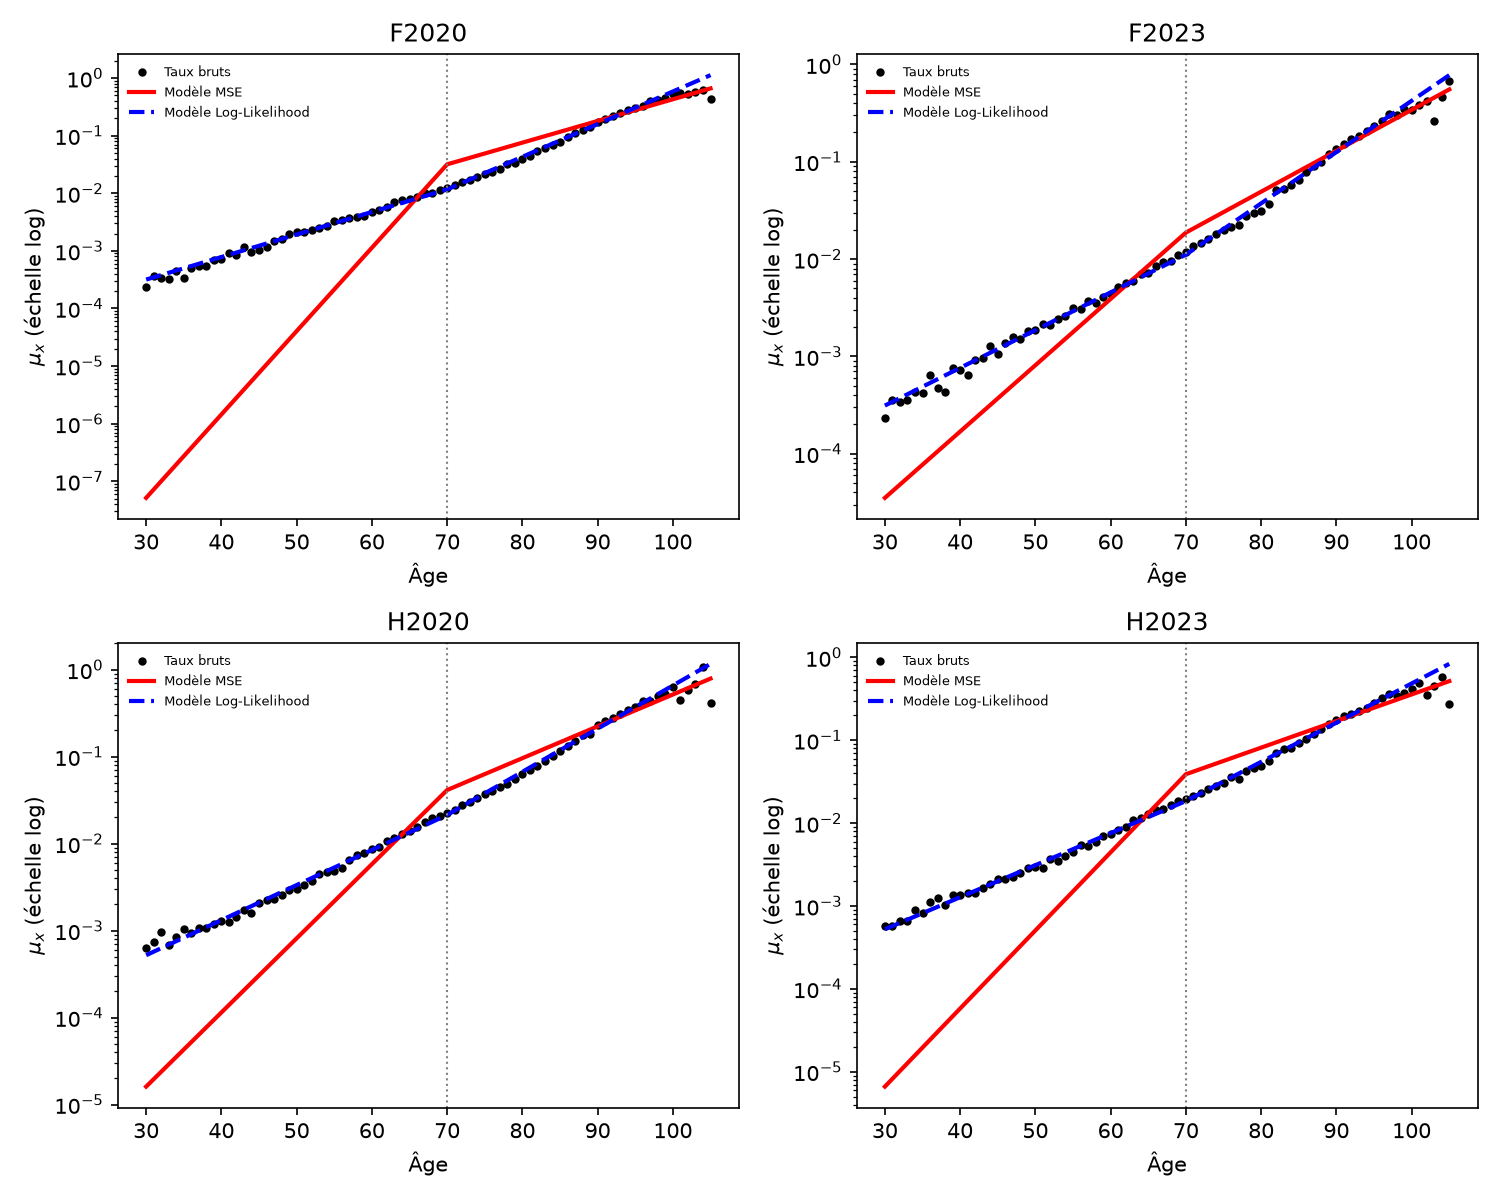
\includegraphics[width=\textwidth]{graphique_comparatif_echelle_log.png}
  \caption{Taux bruts et taux du modèle (MSE et log-vraisemblance), échelle logarithmique. La MSE brute est dominée par les grands âges (où $\mux$ est élevé) : le minimum sacrifie l'ajustement aux âges jeunes, ce que l'échelle logarithmique rend très visible. La ligne pointillée verticale indique $x=70$.}
  \label{fig:log}
\end{figure}

\subsubsection{Espérances de vie}

L'espérance de vie complète à l'âge $x$ est
\[
e_x=\int_0^{\infty}{}_tp_x\,dt \;\approx\; \sum_{k=0}^{105-x-1}{}_kp_x\;\frac{1-e^{-\mu_{x+k}}}{\mu_{x+k}} .
\]
Pour justifier le facteur, on intègre sur l'année $[k,k+1[$ la survie ${}_tp_x={}_kp_x\,e^{-\mu_{x+k}(t-k)}$ :
\[
\int_k^{k+1}{}_kp_x\,e^{-\mu_{x+k}(t-k)}\,dt={}_kp_x\;\frac{1-e^{-\mu_{x+k}}}{\mu_{x+k}} .
\]
La somme est tronquée à 105 ans, aussi bien pour le modèle que pour les taux bruts, de sorte que la comparaison reste équitable. Le tableau~\ref{tab:esp_mse} donne les valeurs obtenues pour $x=40,50,60,70$.

\begin{tabular}{lrrrr}
\toprule
 & e40 & e50 & e60 & e70 \\
\midrule
F2020 & 41.74 & 31.74 & 21.81 & 12.98 \\
F2023 & 43.71 & 33.85 & 24.36 & 16.01 \\
H2020 & 38.47 & 28.57 & 19.08 & 11.34 \\
H2023 & 39.84 & 29.90 & 20.28 & 12.38 \\
\bottomrule
\end{tabular}


% =====================================================================
\subsection{Ajustement par maximisation de la log-vraisemblance gaussienne}
% =====================================================================

\subsubsection{Méthode}

Nous supposons que les taux bruts sont gaussiens :
\[
\muhat \sim \mathcal N\big(\mux,\ \sigma_x^2\big), \qquad \sigma_x^2=\frac{\mux}{E_x}.
\]
Cette variance découle de $D_x\sim\mathrm{Poisson}(\mux E_x)$, d'où $\mathrm{Var}(\muhat)=\mathrm{Var}(D_x)/E_x^2=\mux/E_x$. La log-vraisemblance à maximiser est
\[
\ell(a,b,c)=-\frac12\sum_{x=30}^{105}\left[\ln\!\big(2\pi\sigma_x^2\big)+\frac{\big(\muhat-\mux\big)^2}{\sigma_x^2}\right].
\]
Comme $\sigma_x^2$ dépend des paramètres, cette fonction n'est pas un simple critère des moindres carrés pondérés. Si la variance $\sigma^2$ était constante, la maximisation de $\ell$ serait équivalente à la minimisation de la MSE. C'est donc le choix d'une variance proportionnelle à $\mux/E_x$ qui introduit la différence entre les deux méthodes : chaque âge est pondéré par $E_x/\mux$, ce qui équivaut à raisonner en erreurs \emph{relatives} et redonne du poids aux âges jeunes.

\subsubsection{Résultats}

\begin{tabular}{lrrr}
\toprule
 & a & b & c \\
\midrule
F2020 & -10.7575 & 0.0901 & 0.0405 \\
F2023 & -10.7502 & 0.0893 & 0.0321 \\
H2020 & -10.3439 & 0.0928 & 0.0214 \\
H2023 & -10.2265 & 0.0891 & 0.0198 \\
\bottomrule
\end{tabular}


Le tableau~\ref{tab:comp_mse} compare la MSE obtenue avec les paramètres de chaque méthode : par construction la MSE est plus faible pour les paramètres de la méthode MSE, mais l'écart de qualité d'ajustement visible sur la figure~\ref{fig:log} n'apparaît pas dans ce critère.

\begin{table}[htbp]
\caption{MSE obtenue avec les paramètres issus de la minimisation de la MSE et de la log-vraisemblance.}
\label{tab:comp_mse}
\begin{tabular}{lrr}
\toprule
 & MSE & MSE\_via\_likelihood \\
\midrule
F2020 & 0.001362 & 0.010193 \\
F2023 & 0.000845 & 0.002865 \\
H2020 & 0.004208 & 0.010326 \\
H2023 & 0.001472 & 0.006187 \\
\bottomrule
\end{tabular}
\end{table}


% À COMPLÉTER (recommandé) : tableau des valeurs de -log-vraisemblance.
% Valeurs vérifiées (-l au maximum / -l avec les paramètres MSE) :
% F2020 : -319,0 / 424 331 ; F2023 : -324,5 / 2 834 ; H2020 : -339,2 / 15 626 ; H2023 : -343,6 / 29 189
% Idéalement, ajoute leur calcul dans partie_statique.py et exporte-les en .tex.

\subsubsection{Espérances de vie et comparaison}

\begin{tabular}{lrrrr}
\toprule
 & e40 & e50 & e60 & e70 \\
\midrule
F2020 & 43.74 & 34.20 & 25.06 & 16.54 \\
F2023 & 44.77 & 35.24 & 26.10 & 17.59 \\
H2020 & 39.54 & 30.25 & 21.57 & 13.84 \\
H2023 & 41.02 & 31.72 & 23.00 & 15.16 \\
\bottomrule
\end{tabular}


Pour juger la qualité des deux méthodes, nous comparons les espérances de vie estimées à celles calculées directement avec les taux bruts (tableau~\ref{tab:esp_brutes}) et nous en déduisons les biais (estimé moins observé).

\begin{tabular}{lrrrr}
\toprule
 & e40 & e50 & e60 & e70 \\
\midrule
F2020 & 43.76 & 34.21 & 25.08 & 16.67 \\
F2023 & 44.80 & 35.26 & 26.13 & 17.69 \\
H2020 & 39.61 & 30.27 & 21.55 & 13.95 \\
H2023 & 41.08 & 31.78 & 22.98 & 15.25 \\
\bottomrule
\end{tabular}


\begin{tabular}{lrrrr}
\toprule
 & e40 & e50 & e60 & e70 \\
\midrule
F2020 & -2.02 & -2.47 & -3.27 & -3.69 \\
F2023 & -1.09 & -1.41 & -1.77 & -1.68 \\
H2020 & -1.14 & -1.70 & -2.47 & -2.61 \\
H2023 & -1.24 & -1.88 & -2.70 & -2.87 \\
\bottomrule
\end{tabular}


\begin{tabular}{lrrrr}
\toprule
 & e40 & e50 & e60 & e70 \\
\midrule
F2020 & -0.02 & -0.01 & -0.02 & -0.13 \\
F2023 & -0.03 & -0.02 & -0.03 & -0.10 \\
H2020 & -0.07 & -0.02 & 0.02 & -0.11 \\
H2023 & -0.06 & -0.06 & 0.02 & -0.09 \\
\bottomrule
\end{tabular}


\begin{table}[htbp]
\caption{Écart (log-vraisemblance moins MSE) sur les espérances de vie (en années).}
\label{tab:ecart_esp}
\begin{tabular}{lrrrr}
\toprule
 & e40 & e50 & e60 & e70 \\
\midrule
F2020 & 2.00 & 2.46 & 3.25 & 3.56 \\
F2023 & 1.06 & 1.39 & 1.74 & 1.58 \\
H2020 & 1.07 & 1.68 & 2.49 & 2.50 \\
H2023 & 1.18 & 1.82 & 2.72 & 2.78 \\
\bottomrule
\end{tabular}
\end{table}


\textbf{Conclusions.}
\begin{itemize}
  \item Avec la méthode MSE, l'espérance de vie est \emph{sous-estimée} pour les quatre jeux et tous les âges, de $1{,}1$ à $3{,}7$ ans (par exemple $-2{,}02$ an à 40 ans et $-3{,}69$ ans à 70 ans pour F2020).
  \item Avec la log-vraisemblance, les biais sont de l'ordre de $-0{,}02$ à $-0{,}13$ an : le modèle reproduit les espérances de vie observées à quelques jours près.
  \item L'écart entre les deux méthodes vient de l'ajustement aux âges jeunes et moyens : la MSE brute, dominée par les grands âges, laisse le modèle trop élevé aux âges moyens, ce qui diminue l'espérance de vie.
  \item La log-vraisemblance est donc la méthode la plus appropriée pour ce modèle. % À adapter à ta formulation
\end{itemize}

% =====================================================================
\subsection{Tarification de rentes viagères temporaires}
% =====================================================================

\subsubsection{Méthode}

Nous tarifions une rente viagère temporaire de $1\,000$ euros par an, payable en fin d'année, d'une durée de $n=20$ ans, avec un taux technique $i=1{,}25\,\%$ et $v=1/(1+i)$, pour une femme d'âge $x=50, 60, 70$ ans en 2020 et en 2023 :
\[
P_x = 1\,000\sum_{k=1}^{20} v^{\,k}\;{}_kp_x ,\qquad {}_kp_x=\exp\!\Big(-\sum_{j=0}^{k-1}\mu_{x+j}\Big).
\]
Cela donne 12 prix (2 méthodes $\times$ 2 années $\times$ 3 âges). Les prix légaux sont calculés avec la table de mortalité réglementaire XR :
\[
P_x^{\mathrm{XR}} = 1\,000\sum_{k=1}^{20} v^{\,k}\;\frac{\ell_{x+k}}{\ell_x} .
\]
% À COMPLÉTER : justifier le choix de XR (art. 24 §5 a) de l'arrêté royal) et mentionner que FR est autorisée, ce que le professeur a confirmé.

\subsubsection{Résultats}

\begin{tabular}{lrrr}
\toprule
 & x = 50 & x = 60 & x = 70 \\
\midrule
F2020 & 17378.47 & 15280.65 & 10661.24 \\
F2023 & 17095.17 & 15627.76 & 12526.28 \\
\bottomrule
\end{tabular}


\begin{tabular}{lrrr}
\toprule
 & x = 50 & x = 60 & x = 70 \\
\midrule
F2020 & 16960.87 & 16005.81 & 13233.44 \\
F2023 & 16984.21 & 16091.53 & 13634.76 \\
\bottomrule
\end{tabular}


\begin{tabular}{lrrr}
\toprule
 & x = 50 & x = 60 & x = 70 \\
\midrule
MSE F2020 & 17378.47 & 15280.65 & 10661.24 \\
MSE F2023 & 17095.17 & 15627.76 & 12526.28 \\
LL F2020 & 16960.87 & 16005.81 & 13233.44 \\
LL F2023 & 16984.21 & 16091.53 & 13634.76 \\
Table légale XR & 16682.02 & 15384.74 & 12615.36 \\
\bottomrule
\end{tabular}


\subsubsection{Comparaison avec la table légale}

\begin{tabular}{lrrr}
\toprule
 & x = 50 & x = 60 & x = 70 \\
\midrule
F2020 & 4.2 & -0.7 & -15.5 \\
F2023 & 2.5 & 1.6 & -0.7 \\
\bottomrule
\end{tabular}


\begin{tabular}{lrrr}
\toprule
 & x = 50 & x = 60 & x = 70 \\
\midrule
F2020 & 1.7 & 4.0 & 4.9 \\
F2023 & 1.8 & 4.6 & 8.1 \\
\bottomrule
\end{tabular}


\textbf{Conclusions.}
\begin{itemize}
  \item Le modèle MSE donne des prix instables par rapport à XR (de $-15{,}5\,\%$ à $+4{,}2\,\%$) : l'écart de $-15{,}5\,\%$ à 70 ans pour F2020 est un artefact de l'ajustement, pas un résultat économique.
  \item Le modèle log-vraisemblance donne des prix de $1{,}7\,\%$ à $8{,}1\,\%$ supérieurs à XR, et l'écart augmente avec l'âge. La table XR sous-estime donc la survie féminine observée en 2020 et 2023 ; il faut le commenter : % À COMPLÉTER : interprétation (table unisexe, prudence réglementaire, etc.)
  \item % À COMPLÉTER : implication pour un assureur (une rente plus chère est plus prudente pour l'assureur ; une table qui sous-estime la survie conduit à sous-tarifer).
\end{itemize}

% =====================================================================
% Annexe
% =====================================================================
\appendix
\section{Figure complémentaire}

\begin{figure}[H]
  \centering
  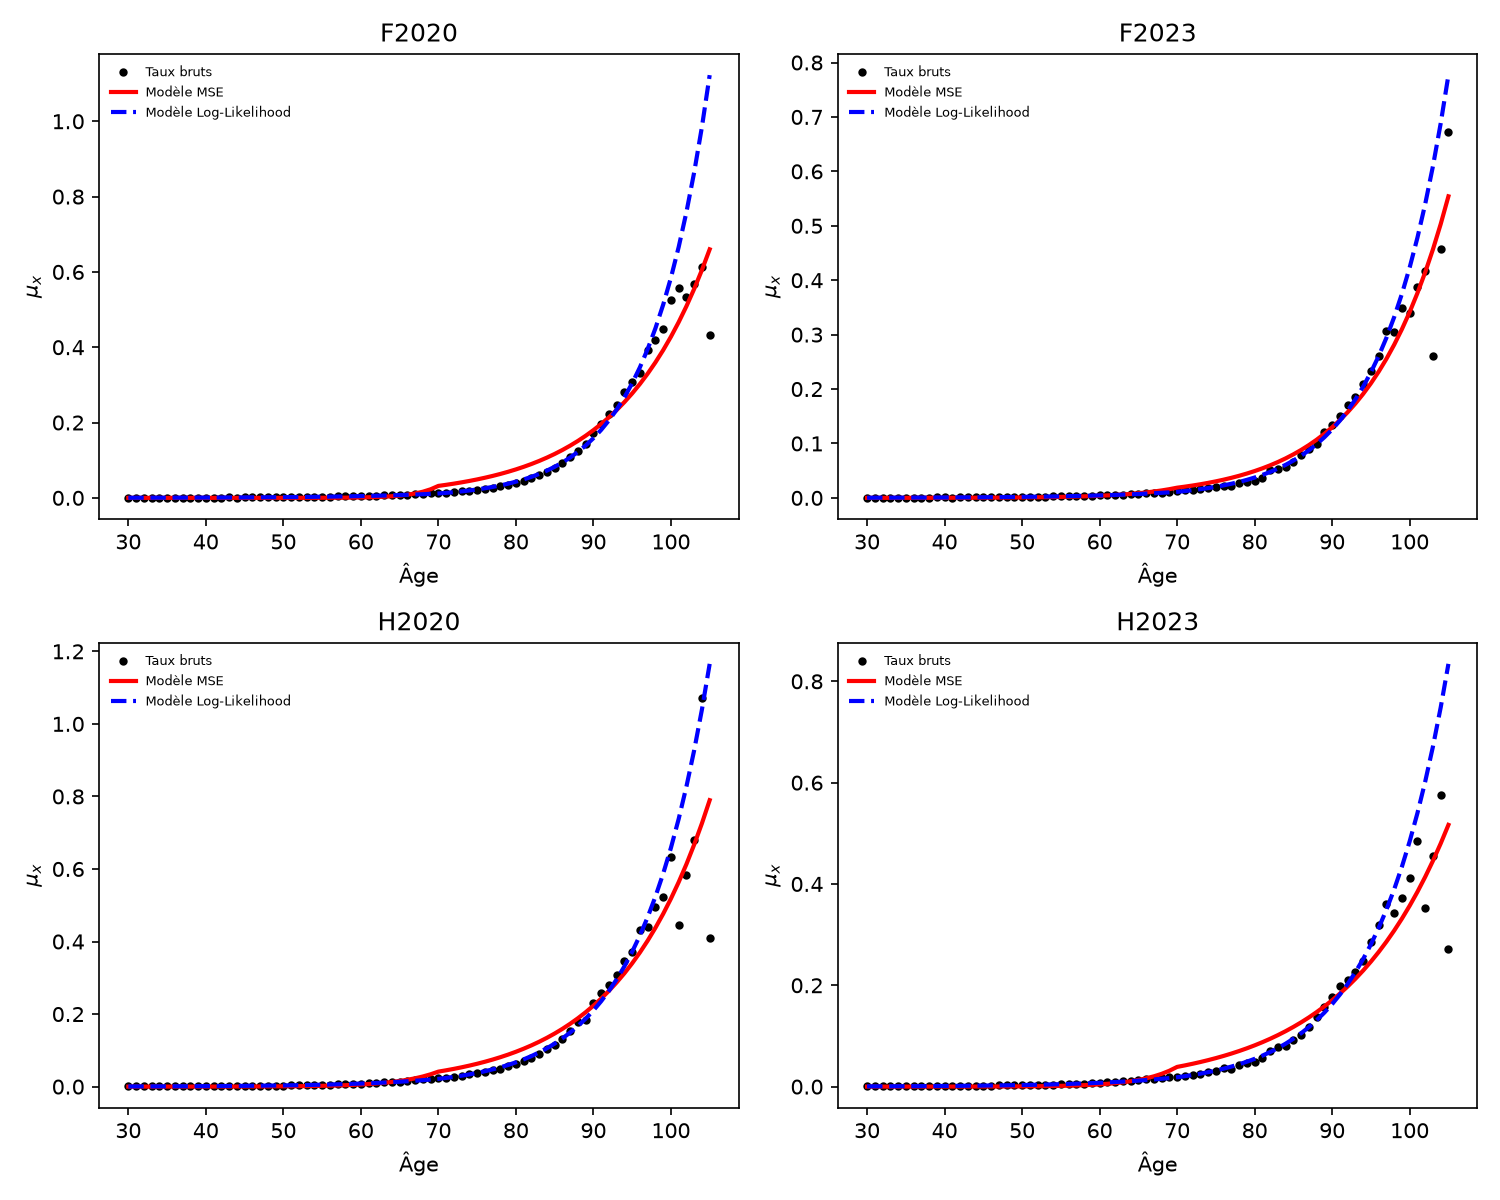
\includegraphics[width=\textwidth]{graphique_comparatif.png}
  \caption{Taux bruts et taux du modèle (MSE et log-vraisemblance), échelle linéaire.}
  \label{fig:lin}
\end{figure}

\end{document}
